% !TEX root = ../my-thesis.tex
%
\chapter{Approach}
\label{sec:approach}

In this chapter, the two alternatives considered in this thesis to tackle the problem of ranking classification algorithms regarding properties of a data set are explained. First, the theoretical approach is presented. Then, implementation details are discussed.

\section{Theory}

In general, the aim is to predict a ranking of algorithms based on properties, or meta features of a data set. This means, that as training data for a ranking approach (ranker), a number of performance values of classifiers need to be recorded on data sets in a first pre-processing phase, for which also meta features are to be computed. The table of this collected data is illustrated in Table \ref{tab:performanceValues}, for n meta features, k classifiers and m data sets. This approach to ranking is realized here, as pointed out before, in a regression-based and preference-based variant, which are explained in detail and compared briefly in the following sections.

\begin{table}[h]
\centering
	\begin{tabularx}{\textwidth}{X | X | X | X | X | X | X | X}
		%\hline
		MF 1			& MF 2		& ... 	& MF n		& PV 1 		& PV 2 		&	...	&	PV k 		\\ \hline
		$v_{11}$		& $v_{12}$	& ...	& $v_{1n}$	& $p_{11}$	& $p_{12}$	& 	...	&	$p_{1k}$		\\ 
		$v_{21}$		& $v_{22}$	& ...	& $v_{2n}$	& $p_{21}$	& $p_{22}$	& 	...	&	$p_{2k}$		\\ 
		...			& ...		& ...	& ...		& ...		& ...		&	...	&	...			\\ 
		$v_{m1}$		& $v_{m2}$	& ... 	& $v_{mn}$	& $p_{m1}$	& $p_{m2}$	& 	...	&	$p_{mk}$			 
	\end{tabularx}
	\caption{Training data for the rankers.}
	\label{tab:performanceValues}
\end{table}

\subsection{Regression-Based Ranking}
% How is the regression ranking done
One possibility to derive a ranking of classifiers from this information when given a new data set is to use regression models. The idea is to use separate regression models to predict a performance value for each classifier, and to subsequently derive an ordering from these predictions. The training of the ranker is done by splitting the data set compiled beforehand (see Tab. \ref{tab:performanceValues}) into separate data sets that each contain all meta features for all data sets, but only the performance values of one classifier, as illustrated in Table \ref{tab:regressionTables}. The target feature on these individual data sets, the performance value of the classifier, is a numeric value, and thus, a regression model is trained on each of them. All regression models therefore try to learn the target function \textit{meta features}$\rightarrow$\textit{performance value} for their respective classifier. After the regression models have been trained for each classifiers, the training of the ranker is finished. For a query instance, here represented by a new data set, the first step is to compute the meta features. Afterwards, these are fed into each regression model and the predicted performance value for each classifier is saved. In a second step, the classifiers are ordered according to the predictions. This generation of a ranking is presented in Figure \ref{fig:regression_ranker_model}.

\begin{table}[h]
\centering
\resizebox{\textwidth}{!}{%
	\begin{tabularx}{1.1\textwidth}{X | X | X | X}
		%\hline
		Meta Feature 1	& ... 	& Meta Feature n		& Performance Value 1	\\ \hline
		$v_{11}$			& ...	& $v_{1n}$			& $p_{11}$				\\ 
		$v_{21}$			& ...	& $v_{2n}$			& $p_{21}$				\\ 
		...				& ...	& ...				& ...					\\ 
		$v_{m1}$			& ... 	& $v_{mn}$			& $p_{m1}$				\\ \hline\hline
		Meta Feature 1	& ... 	& Meta Feature n		& Performance Value 2 	\\ \hline
		$v_{11}$			& ...	& $v_{1n}$			& $p_{12}$				\\ 
		$v_{21}$			& ...	& $v_{2n}$			& $p_{22}$				\\ 
		...				& ...	& ...				& ...					\\ 
		$v_{m1}$			& ... 	& $v_{mn}$			& $p_{m2}$					 
	\end{tabularx}
}	
\vspace{1em}
$\vdots$
\vspace{1em}	
\resizebox{\textwidth}{!}{%
	\begin{tabularx}{1.1\textwidth}{X | X | X | X}
		%\hline
		Meta Feature 1	& ... 	& Meta Feature n		& Performance Value k 	\\ \hline
		$v_{11}$			& ...	& $v_{1n}$			& $p_{1k}$				\\ 
		$v_{21}$			& ...	& $v_{2n}$			& $p_{2k}$				\\ 
		...				& ...	& ...				& ...					\\ 
		$v_{m1}$			& ... 	& $v_{mn}$			& $p_{mk}$					 
	\end{tabularx}
}
	\caption{How the regression ranker processes the training data. Performance data for each classifier are in a separate table, which are then used to train separate regression models.}
	\label{tab:regressionTables}
\end{table}

\begin{figure}
\centering
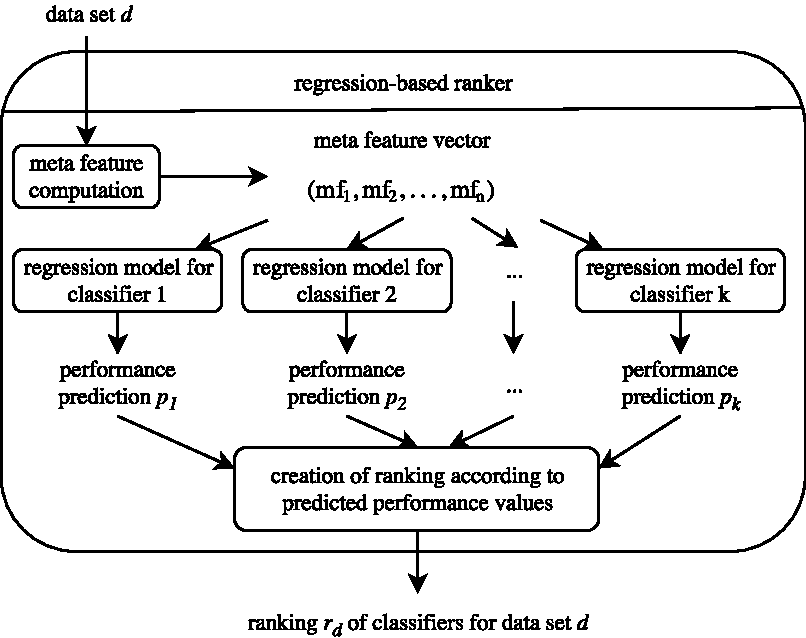
\includegraphics[scale=1]{gfx/regression_models.pdf}
\caption{An overview of how a regression-based ranker constructs a ranking.}
\label{fig:regression_ranker_model}
\end{figure}

\subsection{Preference-Based Ranking}
% How is the preference ranking done
The second possibility considered in this context is using preference learning to predict a ranking. Each instance of the data set generated beforehand (see Tab. \ref{tab:performanceValues}) contains meta feature information for the considered data set and performance values of all classifiers. The performance values can be converted to preference information by sorting the corresponding classifiers by their performance values for each data set, similar to the prediction step of the regression alternative, which is the first step of building the ranker. This leads to an ordering of classifiers associated with each instance, and implies that the preference learning task at hand is label ranking. In this case, in contrast to the regression-based approach, there exists only one model, a label ranking model. To complete the training of the ranker, this model is built with the training data that has been converted to a label ranking data set in the previous step. To make predictions, the computed meta data for a new data set is fed to this model, which consequently returns an ordering of classifiers, which is depicted in Figure \ref{fig:preference_ranker_model}. Thereby, it attempts to learn the mapping from meta features to an ordering of classifiers directly.

\begin{table}[h]
\centering
	\begin{tabularx}{\textwidth}{X | X | X | X | X}
		%\hline
		MF 1				& MF 2				& ... 	& MF n				& Ranking 	\\ \hline
		$v_{11}$			& $v_{12}$			& ...	& $v_{1n}$			& $r_1$		\\ 
		$v_{21}$			& $v_{22}$			& ...	& $v_{2n}$			& $r_2$		\\
		...				& ...				& ...	& ...				& ...		\\
		$v_{m1}$			& $v_{m2}$			& ... 	& $v_{mn}$			& $p_m$		 
	\end{tabularx}
	\label{tab:preferenceTable}
	\caption{How the preference ranker processes the training data. The ranker is trained with a table containing meta features and a ranking of classifiers for each data set.}
\end{table}

\begin{figure}
\centering
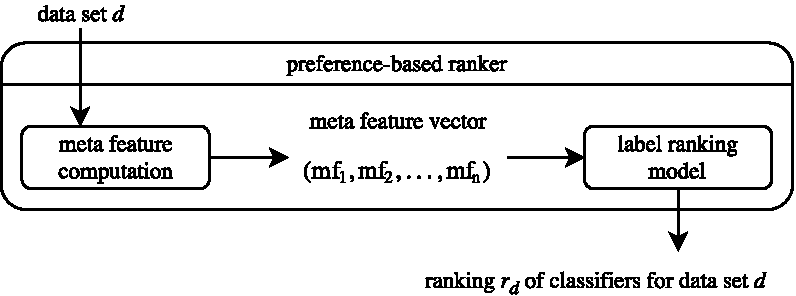
\includegraphics[scale=1]{gfx/label_ranking_model.pdf}
\caption{An overview of how a preference-based ranker constructs a ranking.}
\label{fig:preference_ranker_model}
\end{figure}

\subsection{Comparison}

While both of the ranking approaches above are used for the same purpose of ranking classification algorithms, they differ in some aspects that are interesting to point out. First, they theoretically do not require the same kind of training data. While the preference ranker only needs rankings, the regression ranker requires the exact performance data of all considered classifiers on the data sets. Although here it does not make a difference, since the performance values are computed anyways as the regression ranker utilizes them, in cases where only rankings of classifiers for a data set are known or performance values are estimated in a way that is biased, but has the same bias for all classifiers, so that the ranking is not influenced, this may be an advantage. Furthermore this leads to the curios case that training examples for the regression ranker are not directly samples from the target function the ranker learns. The target function for the regression ranker (as for the preference ranker) maps meta features of a data set to a ranking. However, for the regression ranker, the training examples have to include the actual performance values, meaning that they are of the form (\textit{meta features}, \textit{performance values}). 

Also, the approaches behave differently regarding the addition (or deletion) of a data set or classifier. If a classifier is added, for the regression-based approach, a regression model needs to be added to the ranker. Therefore, performance values for the classifier for the data set would need to be available or have to be computed anew. For the preference-based approach, however, the whole label ranking model, therefore the whole ranker, would need to be trained again, as for every data set, the ranking of classifiers has changed. Here a regression ranker conceptually has an advantage. The deletion of a classifier is much simpler: for the regression-based ranker, one regression model has to be deleted, which does not affect the other models, and in the case of the preference ranker, in the rankings produced by the label ranking model the unwanted classifier can just be removed from the rankings.

For the addition of a data set, the situation is unfavorable for both rankers. Since a new training example would be added to each regression model, they all need to be trained again on the now extended training data. For the preference ranker, likewise a new training example is added to the training data, and a new model has to be trained. The same is the case for the deletion of a data set.

Regarding training and prediction, conceptually, the preference ranker has the advantage that it both only needs to build one model and to have one model make a prediction for a new data set. On the other hand, the regression ranker needs to build as many models as there are classifiers in consideration, and also have as many models predict a performance value for their respective classifiers, which then also have to be turned into a ranking. In general, this indicates a better scalability of the preference-based approach regarding the number of classifiers (unless they are to be added dynamically) and data sets, although of course this also depends on the specific algorithms used. 

\section{Implementation}

The implementation of the rankers themselves is relatively straightforward with the theory of the previous sections in mind. However, since the goals for his thesis includes the development of an AutoML tool that returns a ranking of classification algorithms when given a data sets, the scope of the implementation goes beyond the ranking algorithms, including also pre-processing steps and means of evaluation for the rankers, relevant parts of the implementation are described in the following paragraphs; it is notable that all implementations were carried out in Java, particularly Java 8.

As mentioned before, the implementations of the ranking approaches are relatively close to the theory and will therefore not be described in detail, except for a few notable parts. First, since the tool relies on external libraries for the learning algorithms, these need to be pointed out. For the implementation of the regression models, WEKA was used, a popular libary of machine learning algorithms that includes algorithms for classification, regression, and provides help in the evaluation of these learning algorithms \cite{hall2009weka}. Regarding the preference algorithms, the jPL framework was used \cite{intelligent2017jpl}. The jPL framework is a Java framework for the evaluation of preference learning algorithms, it implements several tasks from the context of preference learning, including label ranking, and also provides a representation for data sets that contain label ranking information. 

Furthermore, so far, the descriptions of the `performance measure' used for the classifiers, that is the measure according to which the classifiers are ranked, for example the error rate or predictive accuracy, have been kept non-specific. Likewise, although the measure used in the evaluation in this thesis is predictive accuracy, the implementation has been kept general to allow any measure to be used with the rankers, as long as it is numeric.

Another fact worth mentioning regarding the implementation of the rankers is that both the regression-based approach and the preference-based approach are implemented in a way that abstract superclasses handle the data set conversions and other necessary tasks, so that it is very easy to add a new ranker implementation. For example, to create a new ranker that uses random forest as a regression model for each classifier, it is only necessary to override a method called \texttt{buildRegressionModels} which has the classifiers mapped to the training data necessary for the regression model of each classifier as a parameter and is responsible for the generation of the regression models. How this method is implemented in the case of random forest is illustrated in Figure \ref{lst:randomForest}. Here we can see that the regression model that has been acquired by training on the provided data is saved together with the classifier for which it predicts performance values. Later, this model is used to predict the performance value of that specific classifier. 

\begin{figure}
\begin{lstlisting}
@Override
protected void buildRegressionModels
			(Map  Classifier, Instances> train) 
			throws Exception {
	regressionModels = new HashMap<Classifier,Classifier>();
	for (Classifier classifier : train.keySet()) {
		RandomForest forest = new RandomForest();
		forest.buildClassifier(train.get(classifier));
		regressionModels.put(classifier, forest);
	}
}
\end{lstlisting}
\caption{A source code excerpt for a ranker based on the random forest algorithm.}
\label{lst:randomForest}
\end{figure}

Last, while the computation of the meta features is included in the workflow of a ranker in the theoretical explanations of the previous sections, meta features are calculated separately in the implementation since it is a repeating task, to speed up the evaluation of classifiers. The list of meta features used is taken from OpenML \cite{OpenML2013}, a website that not only provides a large number of openly accessible data sets, but also records performance values of learning algorithms on these data sets, and features properties of data sets. Thus the meta features were calculated with the help of an implementation provided by OpenML in its Evaluation Engine \cite{openMLEvaluationEngine}; the full list of meta features is included in Table \ref{tab:metaFeatureDetails} in the Appendix. Like the choice which classifier and performance measure to use, the choice of which meta features to be used in the implementation can be changed flexibly.

In addition to this ranking functionality, methods for the evaluation of both classifiers and rankers are implemented. Although WEKA offers capabilities for the evaluation of classifiers, additional functionality had to be added, as for example the desired estimation procedure of stratified Monte Carlo cross-validation was not supported by WEKA at the time of the implementation. Furthermore, since for the evaluation of the rankers (to build the table depicted in Tab. \ref{tab:performanceValues}), many classifiers had to be evaluated on a large number of data sets, an efficient way to execute this task was needed. This was realized by enabling the tool to take a number of jobs, consisting of classifiers and data sets, as command-line parameters, which enables execution for example on a data mining cluster. For the evaluation of rankers, the functionality needed to be built without the help of existing frameworks, and was realized in a similar way to the implemented evaluation of WEKA classifiers. It was also implemented such that after a ranker has been trained once, it can be evaluated regarding a number of different measures, to speed up the evaluation process.

Apart from the functionality described above, the implementation includes some useful recurring functions from the context of handling data sets and classifiers in the context of WEKA and OpenML. To give a general idea how the tool is structured, an overview of the package structure is given in Fig. \ref{fig:package_overview}.

\begin{figure}
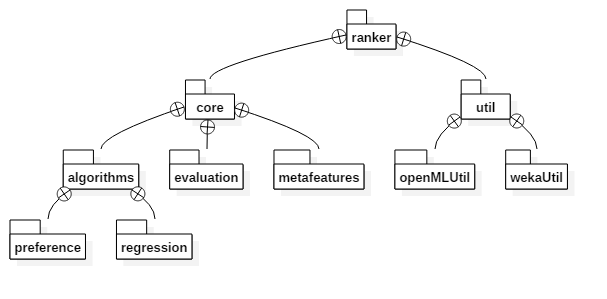
\includegraphics[width=\textwidth]{gfx/Package_Structure.png}
\caption{An overview of the package structure of the tool.}
\label{fig:package_overview}
\end{figure}
